\documentclass[a4paper,11pt,twoside]{memoir}
\chapterstyle{veelo}

\usepackage{TUINFDA}

\usepackage{url}
\usepackage{hyperref}					% links in pdf
\usepackage{graphicx}            			% Figures
\usepackage{verbatim}            			% Code-Environment
\usepackage[lined,linesnumbered,algochapter]{algorithm2e} % Algorithm-Environment

\usepackage{pgf}					
\usepackage{tikz}					% tikz graphics
\usetikzlibrary{arrows,automata}

\usepackage{ngerman}
\usepackage[ngerman]{babel}
\usepackage{bibgerm,cite}       % Deutsche Bezeichnungen, Automatisches Zusammenfassen von Literaturstellen
\usepackage[ngerman]{varioref}  % Querverweise
% to use the german charset include cp850 for MS-DOS, ansinew for Windows and latin1 for Linux.
% \usepackage[latin1]{inputenc}

\thesistitle{Title of the Thesis}
\thesissubtitle{Optional Subtitle} % optional
\thesisdate{TT.MM.JJJJ}

% all titles and designations have to be gender-related!
\thesisdegree{Diplom-Ingenieur}{Diplom-Ingenieur}
\thesiscurriculum{Software Engineering \& Internet Computing}{Software Engineering \& Internet Computing} % your study
\thesisverfassung{Petar Petrov} % Verfasser
\thesisauthor{Petar Petrov} % your name
\thesisauthoraddress{Kochgasse 34, 1080 Wien} % your address
\thesismatrikelno{0508142} % your registration number

\thesisbetreins{Ao.Univ.Prof. Dipl.-Ing. Dr.techn. Andreas Rauber, Univ. Doz.}
\thesisbetrzwei{Dr. Christoph Becker}
%\thesisbetrdrei{Dr. Vorname Familienname} % optional

% define page numbering styles
\makepagestyle{numberCorner}
\makeevenfoot{numberCorner}{\thepage}{}{}
\makeoddfoot{numberCorner}{}{}{\thepage}

% define custom macros for specific formats or names
\newcommand{\uml}[1]{\texttt{#1}}
\newcommand{\cd}{\textsf{Class Diagram}}

\begin{document}

\captionnamefont{\bfseries}

%%%%%%%%%%%%%%%%%%%%%%%%%%%%%%%%%%%%%%%%%
%%%   FRONTMATTER    %%%%%%%%%%%%%%%%%%%%
%%%%%%%%%%%%%%%%%%%%%%%%%%%%%%%%%%%%%%%%%
\frontmatter
\pagenumbering{roman}

%%%%%%%%%%%%%%%%%%%%%%%%%%%%%%%%%%%%%%%%%
%%%   TITLEPAGES    %%%%%%%%%%%%%%%%%%%%%
%%%%%%%%%%%%%%%%%%%%%%%%%%%%%%%%%%%%%%%%%

% the german title page is required as first page
% $Id: titlepage.tex 1752 2010-03-20 11:07:02Z tkren $
%
% TU Wien - Faculty of Informatics
% thesis titlepage
%
% This titlepage is using the geometry package, see
% <http://www.ctan.org/macros/latex/contrib/geometry/geometry.pdf>
%
% For questions and comments send an email to
% Thomas Krennwallner <tkren@kr.tuwien.ac.at>
% or to Petra Brosch <brosch@big.tuwien.ac.at>
%

\selectlanguage{ngerman}

% setup page dimensions for titlepage
\newgeometry{left=2.4cm,right=2.4cm,bottom=2.5cm,top=2cm}

% force baselineskip and parindent
\newlength{\tmpbaselineskip}
\setlength{\tmpbaselineskip}{\baselineskip}
\setlength{\baselineskip}{13.6pt}
\newlength{\tmpparindent}
\setlength{\tmpparindent}{\parindent}
\setlength{\parindent}{17pt}

% first titlepage
\thispagestyle{tuinftitlepage}

%
% Kludge: for each titlepage set \pagenumbering to a different
% style. This is used to fix a problem with hyperref, because there
% are multiple "page 1" and hyperref hates that
%
\pagenumbering{Alph}

\begin{center}
{\ \vspace{3.4cm}}

\begin{minipage}[t][2.8cm][s]{\textwidth}%
\centering
\thesistitlefontHUGE\sffamily\bfseries\tuinfthesistitle\\
\bigskip
{\thesistitlefonthuge\sffamily\bfseries\tuinfthesissubtitle}
\end{minipage}

\vspace{1.3cm}

{\thesistitlefontLARGE\sffamily \tuinfthesistype}

\vspace{6mm}

{\thesistitlefontlarge\sffamily zur Erlangung des akademischen Grades}

\vspace{6mm}

{\thesistitlefontLARGE\sffamily\bfseries \tuinfthesisdegree}

\vspace{6mm}

{\thesistitlefontlarge\sffamily im Rahmen des Studiums}

\vspace{6mm}

{\thesistitlefontLarge\sffamily\bfseries \tuinfthesiscurriculum}

\vspace{6.5mm}

{\thesistitlefontlarge\sffamily eingereicht von}

\vspace{6mm}

{\thesistitlefontLarge\sffamily\bfseries \tuinfthesisauthor}

\vspace{1.5mm}

{\thesistitlefontlarge\sffamily Matrikelnummer \tuinfthesismatrikelno} 

\vspace{1.4cm}

\vspace{0pt}\raggedright\thesistitlefontnormalsize\sffamily
\begin{minipage}[t][1.6cm][t]{\textwidth}%
  %
  an der

  Fakult\"{a}t f\"{u}r Informatik der Technischen Universit\"{a}t Wien
\end{minipage}

\begin{minipage}[t][4cm][t]{\textwidth}%
  \vspace{0pt}\raggedright\thesistitlefontnormalsize\sffamily
  %
  \begin{tabbing}%
	    \hspace{19mm} \= \hspace{66mm} \kill
	    \tuinfthesisbetreuung: \> \tuinfthesisbetreins\\
	    Mitwirkung: \> \tuinfthesisbetrzwei\\
	                \> \tuinfthesisbetrdrei
  \end{tabbing}
\end{minipage}

\begin{minipage}[t][1.5cm][t]{\textwidth}%
  \vspace{0pt}\sffamily\thesistitlefontnormalsize
  \begin{tabbing}%
    \hspace{45mm} \= \hspace{63mm} \= \hspace{51mm} \kill
    Wien, \tuinfthesisdate \> {\raggedright\rule{51mm}{0.5pt}} \> {\raggedright\rule{51mm}{0.5pt}} \\
    \> \begin{minipage}[t][0.5cm][t]{51mm}\centering (Unterschrift \tuinfthesisverfassung)\end{minipage}
    \> \begin{minipage}[t][0.5cm][t]{51mm}\centering (Unterschrift \tuinfthesisbetreuung)\end{minipage}
    \end{tabbing}
\end{minipage}

\end{center}

% we want an empty page right after first titlepage
\pagestyle{empty}
\cleardoublepage

% we're done with the titlepages, proceed with default pagenumbering
\pagenumbering{roman}

% restore baselineskip
\setlength{\baselineskip}{\tmpbaselineskip}
\setlength{\parindent}{\tmpparindent}

% back to normal geometry
\restoregeometry

\selectlanguage{english}

%%% Local Variables:
%%% TeX-PDF-mode: t
%%% TeX-debug-bad-boxes: t
%%% TeX-parse-self: t
%%% TeX-auto-save: t
%%% reftex-plug-into-AUCTeX: t
%%% End:


% an english translation may follow
% $Id: titlepage.tex 1752 2010-03-20 11:07:02Z tkren $
%
% TU Wien - Faculty of Informatics
% thesis titlepage
%
% This titlepage is using the geometry package, see
% <http://www.ctan.org/macros/latex/contrib/geometry/geometry.pdf>
%
% For questions and comments send an email to
% Thomas Krennwallner <tkren@kr.tuwien.ac.at>
% or to Petra Brosch <brosch@big.tuwien.ac.at>
%

% setup page dimensions for titlepage
\newgeometry{left=2.4cm,right=2.4cm,bottom=2.5cm,top=2cm}

% force baselineskip and parindent
%\newlength{\tmpbaselineskip}
%\setlength{\tmpbaselineskip}{\baselineskip}
%\setlength{\baselineskip}{13.6pt}
%\newlength{\tmpparindent}
%\setlength{\tmpparindent}{\parindent}
%\setlength{\parindent}{17pt}

% first titlepage
\thispagestyle{tuinftitlepage}

%
% Kludge: for each titlepage set \pagenumbering to a different
% style. This is used to fix a problem with hyperref, because there
% are multiple "page 1" and hyperref hates that
%
\pagenumbering{Roman}

\begin{center}
{\ \vspace{3.4cm}}

\begin{minipage}[t][2.8cm][s]{\textwidth}%
\centering
\thesistitlefontHUGE\sffamily\bfseries\tuinfthesistitle\\
\bigskip
{\thesistitlefonthuge\sffamily\bfseries\tuinfthesissubtitle}
\end{minipage}

\vspace{1.3cm}

{\thesistitlefontLARGE\sffamily \tuinfthesistypeen}

\vspace{6mm}

{\thesistitlefontlarge\sffamily submitted in partial fulfillment of the requirements for the degree of}

\vspace{6mm}

{\thesistitlefontLARGE\sffamily\bfseries \tuinfthesisdegreeen}

\vspace{6mm}

{\thesistitlefontlarge\sffamily in}

\vspace{6mm}

{\thesistitlefontLarge\sffamily\bfseries \tuinfthesiscurriculumen}

\vspace{6.5mm}

{\thesistitlefontlarge\sffamily by}

\vspace{6mm}

{\thesistitlefontLarge\sffamily\bfseries \tuinfthesisauthor}

\vspace{1.5mm}

{\thesistitlefontlarge\sffamily Registration Number \tuinfthesismatrikelno} 

\vspace{1.4cm}

\begin{minipage}[t][1.6cm][t]{\textwidth}%
  \vspace{0pt}\raggedright\thesistitlefontnormalsize\sffamily
  %
  to the Faculty of Informatics 

  at the Vienna University of Technology
\end{minipage}

\vspace{0pt}\raggedright\thesistitlefontnormalsize\sffamily
\begin{minipage}[t][4cm][t]{\textwidth}%
  \begin{tabbing}%
	    \hspace{19mm} \= \hspace{66mm} \kill
	    Advisor: \> \tuinfthesisbetreins\\
	    Assistance: \> \tuinfthesisbetrzwei\\
	                \> \tuinfthesisbetrdrei
     \end{tabbing}
\end{minipage}

\begin{minipage}[t][1.5cm][t]{\textwidth}%
  \vspace{0pt}\sffamily\thesistitlefontnormalsize
  \begin{tabbing}%
    \hspace{45mm} \= \hspace{63mm} \= \hspace{51mm} \kill
    Vienna, \tuinfthesisdate \> {\raggedright\rule{51mm}{0.5pt}} \> {\raggedright\rule{51mm}{0.5pt}} \\
    \> \begin{minipage}[t][0.5cm][t]{51mm}\centering (Signature of Author)\end{minipage}
    \> \begin{minipage}[t][0.5cm][t]{51mm}\centering (Signature of Advisor)\end{minipage}
    \end{tabbing}
\end{minipage}

\end{center}

% we want an empty page right after first titlepage
\pagestyle{empty}
\cleardoublepage

% we're done with the titlepages, proceed with default pagenumbering
\pagenumbering{roman}

% restore baselineskip
\setlength{\baselineskip}{\tmpbaselineskip}
\setlength{\parindent}{\tmpparindent}

% back to normal geometry
\restoregeometry


%%% Local Variables:
%%% TeX-PDF-mode: t
%%% TeX-debug-bad-boxes: t
%%% TeX-parse-self: t
%%% TeX-auto-save: t
%%% reftex-plug-into-AUCTeX: t
%%% End:
 % optional

%%%%%%%%%%%%%%%%%%%%%%%%%%%%%%%%%%%%%%%%%
%%%   ERKLAERUNG DER SELBSTAENDIGKEIT   %
%%%%%%%%%%%%%%%%%%%%%%%%%%%%%%%%%%%%%%%%%
\cleardoublepage
\selectlanguage{ngerman}
\chapter*{Erklärung zur Verfassung der Arbeit}

\tuinfthesisauthor\\
\tuinfthesisauthoraddress

\vspace*{1.2cm}

Hiermit erkläre ich, dass ich diese Arbeit selbständig verfasst habe, 
dass ich die verwendeten Quellen und Hilfsmittel vollständig angegeben 
habe und dass ich die Stellen der Arbeit - einschließlich Tabellen, 
Karten und Abbildungen -, die anderen Werken oder dem Internet im 
Wortlaut oder dem Sinn nach entnommen sind, auf jeden Fall unter Angabe 
der Quelle als Entlehnung kenntlich gemacht habe.\\

\vspace*{2cm}
\begin{tabbing}%
    \hspace{58mm} \= \hspace{28mm} \= \hspace{58mm} \kill
    {\raggedright\rule{58mm}{0.5pt}} \> \> {\raggedright\rule{58mm}{0.5pt}} \\
    \begin{minipage}[t][0.5cm][t]{58mm}
	\vspace{0pt}\sffamily\thesistitlefontnormalsize
	\centering (Ort, Datum)
    \end{minipage}
    \> \>
    \begin{minipage}[t][0.5cm][t]{58mm}
	\vspace{0pt}\sffamily\thesistitlefontnormalsize
	\centering (Unterschrift \tuinfthesisverfassung)
    \end{minipage}
\end{tabbing}


\selectlanguage{english}

%%%%%%%%%%%%%%%%%%%%%%%%%%%%%%%%%%%%%%%%%
%%%   ACKNOWLEDGEMENTS    %%%%%%%%%%%%%%%
%%%%%%%%%%%%%%%%%%%%%%%%%%%%%%%%%%%%%%%%%

% optional acknowledgements may be included in german or in english
%\chapter*{Danksagung}

Hier fügen Sie optional eine Danksagung ein.
 		% optional
\chapter*{Acknowledgements}
Part of the following  work was supported by the European Union in the 7th Framework Program, IST, through the SCAPE project, Contract 270137. \newline\newline

I would like to thank my supervisor, Prof. Andreas Rauber, for the insightful and inspirational conversations, the helpful comments and constructive suggestions, as well as for giving me the opportunity to work with one of the best people in the digital preservation community and letting me be part of his team and the SCAPE project.

I also would like to thank my other supervisor and reviewer, Dr. Christoph Becker, for his guidance, technical support and suggestions during the creation of this document and the prototype implemented as part of this work. Without him, everything presented here would have never been a part of the SCAPE project and I probably wouldn't have written it, as he inspired me and encouraged me to do so. I thank him for all those critical, but constructive reviews and talks that sometimes made my life seem hard but without which this thesis wouldn't be. I also thank him for helping me disseminate this work and supporting me throughout many long meetings and heated discussions with other partners within the project.

Last but not least, I would like to thank my family not only for supporting my studies abroad financially, but also for providing me with good example and for always being there for me offering help and good advice.\newline\newline

Thank You!	% optional

%%%%%%%%%%%%%%%%%%%%%%%%%%%%%%%%%%%%%%%%%
%%%   ABSTARCT    %%%%%%%%%%%%%%%%%%%%%%%
%%%%%%%%%%%%%%%%%%%%%%%%%%%%%%%%%%%%%%%%%

\chapter*{Abstract}
Information Technology enables us to organize our digital content into collections of objects in an easy fashion and thus massive volumes of data are produced each day.
However it opens up a huge set of technical and social issues regarding its safety and long-term accessibility \cite{Lorie:2001:LTP:379437.379726}.

Digital Preservation copes with such issues related to hardware and software obsolescence. Among its various
options are tools like emulation, bit-stream and logical preservation. In order to make a meaningful decision
about the potential alternatives or preservation actions that should or should not be executed on a
digital collection, preservation planning is conducted. A preservation plan specifies a concrete action plan for the preservation
of a certain set of objects or a collection and includes potential alternatives and reasons for the decision making  \cite{Becker:2009fk}. 

As collections, which have to be preserved in practice are often huge (in the order of tera- and even petabytes consisting of millions of objects) it is not feasible to create a plan based on experiments over the entire collection. For this reason, inarguably one of the most important parts of preservation planning is the description of the collection or in other words the content profile. In general, the process of content profiling consists of three parts; characterization, aggregation and analysis. Characterization is responsible for the extraction of meta data and the identification of digital objects, while aggregation offers a compressed view on them. In the last step of analysis, relevant aspects of the content are found and presented for further processing by preservation planning. Thus the process of content profiling shall give a more detailed description about a collection, as a profile consists not only of simple measures such as size, count of objects and format but also provides a deeper view based on any other feature and its distribution, that is of interest for preservation planning.

Another crucial task that can only be done with a solid content profile is the selection of a meaningful and valid representative subset of a collection \cite{Becker:2011:PDT:1998076.1998089, Pan05findingrepresentative}. Only with such a representative collection of sample objects a planner 
has the needed basis to conduct valid experiments and back up her decisions when choosing the best
preservation action alternative. What is more, evidence for the validity and effectiveness of the considered preservation actions can be easily found, based on the representative subset.

In this thesis we observe the existing gap in terms of content profiling and its importance within preservation
planning. 
%Digital content repositories, such as ESciDoc\footnote{https://www.escidoc.org/} and EPrints\footnote{http://www.eprints.org/} are used to store massive volumes of data, however there is no possiblity for large scale data analysis over the content stored and only simple measures such as number of objects and content types are provided. Thus a content profiling capability in such repositories would serve as a valuable input to preservation planning processes. 
We present a concept for the process of content profiling and a software prototype implementing it.
 %that shall form the basis of an advanced collection profiling step for the preservation planning tool PLATO\footnote{http://ifs.tuwien.ac.at/dp/plato} as presented in \cite{Rauber:2009:dpchallenges}.
 We provide a simple representative set algorithm as a part of the prototype and evaluate it over bigger data collections in two use case studies.
\cleardoublepage
\selectlanguage{ngerman}
\chapter*{Kurzfassung}
\vspace{-1cm}
Informationstechnologien helfen uns unsere digitalen Inhalte (Dokumente, Bilder, etc.) leicht zu verwalten.
Dies ist der Grund f\"{u}r die zur Zeit bemerkenswerte digitale Datenproduktion.
Allerdings, werden dadurch viele technische, sowie auch soziale Probleme, die mit der Sicherheit, Langzeitarchivierung und Zugriff zu tun haben, verursacht.

Digitale Langzeitarchivierung versucht genau diese Probleme zu l\"{o}sen, die mit Hardware- und Softwareveralterung zu tun haben, sowie auch den Zugriff f\"{u}r l\"{a}ngere Zeitr\"{a}ume zu garantieren.
Unter den zahlreichen Optionen stechen Konzepte wie physische und logische Pr\"{a}servierung mit deren unterschiedlichen Auspr\"{a}gungen besonders heraus.

Damit man eine gute Entscheidung \"{u}ber die potentielle Alternativen oder Pr\"{a}servierungsaktionen, die man auf eine digitale Kollektion durchf\"{u}hren oder nicht durchf\"{u}hren sollte, treffen kann, muss man ein Planungsprozess befolgen.
Dies ist ein komplexer Prozess, der ziemlich zeitraubend ist, der aber als Ergebnis ein Pr\"{a}servierungsplan hat.
Der Plan spezifiziert konkrete Aktionen f\"{u}r die Pr\"{a}servierung von einer Menge von digitalen Objekten und umfasst potentielle Alternativen und Gr\"{u}nde f\"{u}r die getroffene Entscheidung.
Da die zu bewahrenden Kollektionen in der Praxis ziemlich gro{\ss} sind (tera oder sogar petabytes, bestehend aus Millionen von Objekten), ist es nicht m\"{o}glich einen Plan zu erstellen, der auf Experimente \"{u}ber die ganze Kollektion basiert.
Aus diesem Grund ist die Erstellung einer umfassenden Beschreibung der Kollektion unbestreitbar einer der wichtigsten Teile des Plannungsprozesses.
Der Prozess der Erstellung von dieser Beschreibung nennt man Content Profiling.

Generell besteht Content Profiling aus drei Teile; Charakterisierung, Aggregation und Analyse.
Im ersten Schritt wird eine Identifikation der digitalen Objekten durchgef\"{u}hrt, sowie Meta Daten werden extrahiert.
In der Aggregationsphase werden alle gesammelten Daten zusammengefasst, sodass diese in einer kompressierten Form dargestellt werden k\"{o}nnen.
Im letzten Schritt werden interessante Aspekte der Kollektion durch eine tiefgehende Analyse festgestellt und f\"{u}r weitere Behandlung bereitgestellt. 
So wird durch den Content Profiling Prozess eine detaillierte Beschreibung der Daten erfasst, da ein Profil nicht nur aus einfache Messungen, wie Gr\"{o}{\ss}e, Anzahl von Objekten und Formate besteht, aber auch eine ausf\"{u}rliche Ansicht darstellt, die auf jeder beliebigen Charakteristik, oder deren Verteilung, basieren kann.
Wegen des Volumens der Daten, ist die Auswahl von einer kleinen Teilmenge von repr\"{a}sentativen Objekten besonders wichtig.
Daraufbasierend werden Experimente durchgef\"{u}hrt, die Evidenz f\"{u}r die Effektivit\"{a}t und G\"{u}ltigkeit der potentiellen Aktionen bereitstellen.

Nach dem aktuellen Stand der Langzeitarchivierung existiert keine L\"{o}sung, die es erlaubt einen detaillierten Profil von signifikanten Datens\"{a}tzen automatisch zu erstellen, repr\"{a}sentative Teilmengen auszuw\"{a}hlen und diese Informationen in einem semi-strukturierten Format darzustellen.

In dieser Arbeit betrachten wir die existierenden L\"{u}cken im Umfeld von dem Content Profiling und dem Planungprozess.
Der Beitrag dieses Werks besteht darin, eine konzeptionelle L\"{o}sung des Problems, sowie eine Implementierung in Form von einem Prototyp zu erstellen.
Das Prototyp kann auf Kollektionen von vern\"{u}nftigen Gr\"{o}{\ss}en arbeiten und hilft einem, eine tiefgehende Analyse durchzuf\"{u}hren.
Abschlie{\ss}end wird dieses anhand zwei Fallstudien von Datenkollektionen mit signifikanten Volumen evaluiert.


\selectlanguage{english}

%%%%%%%%%%%%%%%%%%%%%%%%%%%%%%%%%%%%%%%%%
%%%   CONTENTS    %%%%%%%%%%%%%%%%%%%%%%%
%%%%%%%%%%%%%%%%%%%%%%%%%%%%%%%%%%%%%%%%%
% uncomment to set document language to german (results in "Inhaltsverzeichnis", "Kapitel", "Abbildung", etc. instead of "Contents", "Chapter", and "Figure"), otherwise the document's language is english
%\selectlanguage{ngerman}

\setcounter{tocdepth}{1}

\cleardoublepage
\pagestyle{numberCorner}
\tableofcontents*

%%%%%%%%%%%%%%%%%%%%%%%%%%%%%%%%%%%%%%%%%
%%%   MAINMATTER    %%%%%%%%%%%%%%%%%%%%%
%%%%%%%%%%%%%%%%%%%%%%%%%%%%%%%%%%%%%%%%%

\mainmatter
\pagenumbering{arabic}
\pagestyle{numberCorner}

%%%%%%%%%%%%%%%%%%%%%%%%%%%%%%%%%%%%%%%%%
\chapter{Introduction}
\label{ch:intro}
%%%%%%%%%%%%%%%%%%%%%%%%%%%%%%%%%%%%%%%%%

This chapter introduces the problem of preserving digital information and gives some perspective of the volume of data we have to deal with. It also gives a motivation for this thesis as well as a summary of the problem of content profiling. Following is the aim of this work and how the problem was approached.

\section{Content \& Digital Preservation}
\label{ch:content_and_digital_preservation}
The information age enables us to produce, transfer and share massive volumes of data freely in an easy fashion. Scientists all over the world conduct complex research experiments and simulations that produce such an enormous amount of information that was unimaginable just a couple of decades ago. In Microsoft Research's book Jim Gray gives a simple example of the order of magnitude of data volume that is going to be produced. The Large Synoptic Survey Telescope\footnote{http://www.lsst.org/lsst/about} will produce around 1.3 petabytes of information only it its first year of operation, which is more than any other telescope in history has produced \cite{Gray:2009:fourthparadigm}.

The World Wide Web has certainly played an important role as a catalyst of this data growth. In order to put this fact into perspective, Intel\textsuperscript{\copyright}\footnote{http://www.intel.com/} has created a famous Infographic presented in figure \ref{fig:intel_oneminute_internet}
As it becomes easier and cheaper to create, edit, manipulate, store and share large amounts of digital objects, people often grow unaware of the problems that arise with the digital content they create.

A single sheet of paper, put in a normal environment, can easily endure a number of decades and will most likely still be readable and accessible and even semantically understandable. A digital object, a file that contains the exact same content, often does not stand a chance of living through the next decade. Hardware failures, software obsolescence, changed environments, lack of backup copies are just a small set of examples of what may occur to digital objects and render a user unable to access them again.

Digital Preservation is aiming to preserve digital content through the years and make it findable, accessible, readable and understandable for periods of time which often surpass the lifetime of hardware and software components \cite{DBLP:journals/dlib/RosenthalRLRM05}. In the last years, a growing awareness of digital preservation problems is seen throughout scientific communities, memory institutions and business enterprises. These create solutions and follow different approaches and apply specific workflows on content in order to tackle many problems on different levels.

Currently, content holding institutions possess huge amounts of data. Web Archives for example crawl and store web sites and related content, such as images, video, style sheet files, etc. National and state archives use digital repositories to preserve their content. However, crawling and storing the bits and bytes represents only one step towards preserving all this content.

Regardless of the origin of the content (web archive, scientific data, personal audio and video collections, etc.), preservation planning has to be done in order to be able to identify and apply the most meaningful course of action and thus ensure the long-term safety and accessibility of each object that was stored. And since content and the environments which we use to manage it are continuously evolving, this process has to be repeated on a regular basis.

\begin{figure}[hb]
\begin{center}
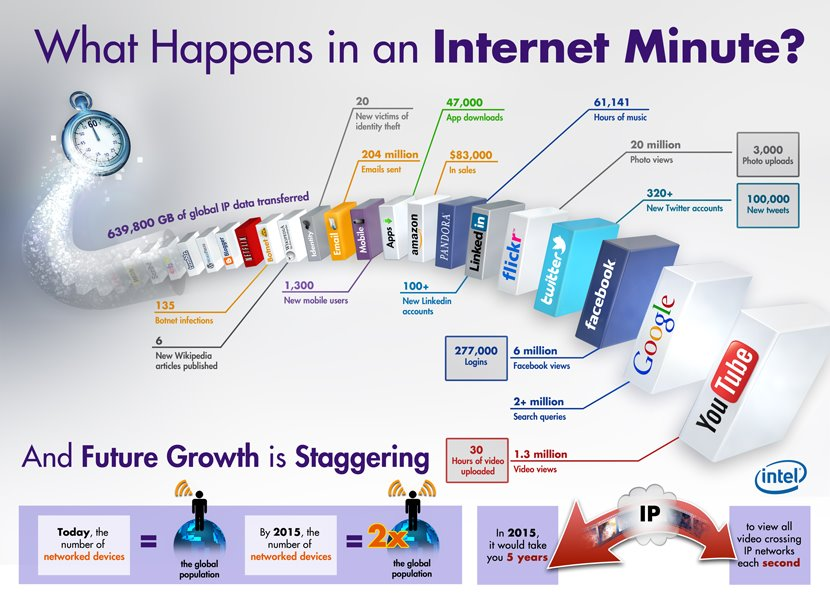
\includegraphics[width=6in]{figures/introduction/intel_oneminute_internet.jpg}
\caption{What happens in an internet minute. (An infographic by Intel\textsuperscript{\copyright})}
\label{fig:intel_oneminute_internet}
\end{center}
\end{figure}

\section{Motivation}
\label{sec:motivation}
% automation and its importance.
% concetrate on collection profiling
% why is it important to know what do we have
% in the collections.
Due to the fast growth and scale of data, the need of automation support in digital preservation processes arises. In order to conduct preservation planning effectively, one has to undertake a well-defined process consisting of numerous steps \cite{Becker:2009fk}. Very important part of this process is the definition of the content that has to be preserved and the representative sample selection. 

The validity and effectiveness of the planning process is highly dependent on a content profile because it defines the scope of the produced plan. A profile defines the content of a collection in terms of its meta data and properties. This meta data plays an important role when preserving digital objects as it not only carries important information about the objects themselves, but also about their structure. Such information provides hints about the digital objects and their type and helps experts decide the best course of action regarding the long-term accesability and preservation of data. A profile also defines a set of sample objects, that are representative to the whole collection of objects. The selected samples provide the basis for the experiments based on which potential courses of action, called preservation alternatives are evaluated. This means that enough valid meta information and knowledge about the content has to be obtained so that only proper alternatives can be chosen. In order to achieve this goal, some very important and necessary steps that provide valuable input to planning have to be undergone. These are currently not always done efficiently, if done at all. For example, the content has to be characterized and all the meta data that is extracted has to be aggregated and analyzed before all potential preservation action alternatives can be found and evaluated. Based on this analysis the content that is to be preserved can be split up into homogeneous sub-collections with similar characteristics and significant properties. Furthermore, such an aggregation of the similarities between different parts of the content can enable more efficient stratification of representative samples in an automatic fashion.

%Based on these and on objective trees defined in another step of the process the most effective preservation action is chosen.
%cite objective tree and representatives.

The presevation planning process is currently done semi-automatically and needs much input regarding the content profile from a preservation expert. Due to the scale of the data a preservation expert often does not have a specific overview of the content profile, but rather high-level knowledge, such as ``The collection consists of 1 million audio files''. It seems that many parts of this process, from characterization to plan deployment and execution, can be automated or at least enhanced by machine processes. Also support for large-scale processing and analysis can be provided by distributed architectures and state of the art algorithms. If this is achieved the effect will be much more valuable than the sum of its parts for the Digital Preservation community.

Nonetheless, the current state of the art does not specify a concrete and well-defined way of how content profiling should be done and what information it should aggregate. What is more, there are almost no evaluation possibilities of the results that characterization tools offer. Some tools try to give confidence level, which is a first step towards such a validation, however it is not enough. A simple example of such uncertainties is character set encoding of html files. Many files specify a UTF-8 encoding, however the real encoding used in the file is different. Some tools are able to detect this, whereas others just report the declared encoding. This is only one of many examples of such uncertainties that arise due to missing quality assurance steps during the characterization process. Such seemingly minor pecularities can cause huge impact on the chosen preservation alternative and thus on the final result of the preserved content. The ability to detect them on a larger scale, to find out subtleties and nuances between different objects in a collection and to select valid representative objects will greatly enhance the preservation planning process.

Thus, a specific way of aggregating large amounts of meta data and its multidimensional representation would be of great value. Only with such a content profile efficient preservation planning can be achieved.

\section{Problem Statement}
\label{sec:problem_statement}
Very often collection and content profiling is done on a very high level, that
is often insufficient for a planning process, especially if this process is to be fully automated.
The current state of the art of content profiling in preservation plans is creating a short description, written by a preservation expert. These descriptions are usualy a very high level assertions, such as: ``The collection contains about 2 million TIFF files''. The profile also contains simple metrics, such as (approximate) collection size, and number of elements as well as the formats identified in the collection. 
These measurements are important but are not the only ones needed for the creation of an efficient preservation plan.
For example, the information about the size of the whole collection is not enough. Other size related measures, such as the overall size of all files in a collection that have a specific format, or the average size of files with a mime type 'text/plain' can be much more significant and helpful in a preservation planning process. Another example where simple measures are not enough are the formats within a collection. In cases of heterogeneous content the distribution of the formats in combination of some other property can turn out to be very helpful for analysis and comprehension of the content. Moreover, in cases of format-homogeneous collections the file format alone will play only a minor role. Combining them with other properties such as the creation date or the creating application could however give deeper insight into the collection.
These are only a few of the examples of multi dimensional characteristics that could turn out to be important in content profiling. However, there are many more that will play different role from case to case.

Furthermore, the creation of a plan has very specific requirements. For example, it needs a small subset of the collection in order to conduct some experiments over it. Based on the results, recommendations and decisions about the preservation actions of the whole collection are produced. Thus the choice of a representative collection subset is a very important process, that is unfortunately often taken lightly, e.g. done randomly or done based on a very shallow analysis. Besides of the manual and random choice of samples in current preservation practices their integration within the planning process is also done manually (either by file upload or manual filling of the related sample information).

Currently, there is no tool that meets these planning requirements and tries to tackle and solve problems arising from the large volume of content, the sparse meta data, the conflicts in the measurements and many other.

The rapid data growth introduces even more problems. In the case of web archives for example, much work has to be done in capturing the significant properties of such dynamic content as the World Wide Web, since the harvested content gets outdated almost immediately after the crawl has been done.

\section{Aim Of The Work}
\label{sec:aim_of_the_work}
In this thesis we aim to analyze the requirements for such a content profiling process and to create a well-defined approach to generate and represent it, so that it can be used as input to other tools, e.g. preservation planning and preservation monitor components.

This will provide a strong basis for preservation planning experts and processes as well as set the foundation for experiments with reduced bias.

The architecture of a software tool that is able to read the characteristics of large amount of files and generate a content profile is to be designed as well as a prototype to be implemented. 

\section{Methodical Approach}
\label{sec:methodical_approach}
In a first step a research of the current methods in scientific projects and institutional practices regarding content profiling will be done. Based on this, a short analysis of the existing gap between the idea of content profiling and the actual steps done will be carried out. 

The main part of the thesis will be the creation of a specification and the architecture of a software tool that is able to profile larger amounts of data and produce output conforming to that specification. In the next step, research about applicable algorithms able to find a (representative) subset of a given collection of characterized digital objects will be performed, and a prototype implementation will be created for the content profiling tool. 

Afterwards a use case study will be conducted, where the produced prototype will be applied on a the Open GovDocs1 collection provided by the Digital Corpora for scientific experiments, which consists of nearly 1 million files and has a total of almost half a terabyte. 

In the last step an evaluation of the tool and the methods applied will be done and based on it a conclusion will be drawn.

\section{Structure Of The Work}
\label{sec:structure_of_the_work}
This thesis is structured as follows: The next chapter offers an overview of digital preservation and preservation planning. The state of the art regarding content profiling is summarized and some observations of the author about the the current related work are discussed. In Chapter 3, a theoretical view of content profiling is presented, where its requirements, issues and open challenges are discussed. Chapter 4 presents the architecture and gives deeper insight into a prototype tool that is designed and implemented as part of this master thesis. The following Chapter 5 describes a use case that was conducted in order to evaluate the tool and draws conclusions about the content profiling approach proposed in this thesis and its implementation. In the last chapter a summary of this thesis is provided as well as the open issues and next steps regarding content profiling that have to be undertaken in future research.

%%%%%%%%%%%%%%%%%%%%%%%%%%%%%%%%%%%%%%%%%
\chapter{Typographic Design}
\label{ch:typo}
%%%%%%%%%%%%%%%%%%%%%%%%%%%%%%%%%%%%%%%%%


For working with LaTeX you can take advantage of a variety of books and free introductions and tutorials on the internet. A competent contact point for LaTeX beginners is the LaTeX Wikibook, which is available under \url{http://en.wikibooks.org/wiki/LaTeX}. 

The following sections give examples of the most important LaTeX environments and commands.

\section{Tables}

Tables have to be realized with the help of the \textit{table} environment. Tables shall be sequentially numbered for each chapter and described in terms of a short caption (cf. Table~\ref{tab:diplomaseminar}).

\begin{table}[htb]
	\centering
	\begin{tabular}{|l|c|c|}
		\hline \textbf{Name} & \textbf{Date} & \textbf{Title} \\
		\hline
		\hline Mustermann Adam  & 18.5   & T1    \\
		\hline Musterfrau Eva  & 22.6   & T2    \\
		\hline
	\end{tabular}
	\caption{Seminar for Master Students}
	\label{tab:diplomaseminar}
\end{table}


\section{Figures}

Like tables, figures shall be sequentially numbered for each chapter and described in terms of a short caption). You could either produce your drawings directly inside Latex using PSTricks\footnote{\url{http://tug.org/PSTricks}}, Tikz\footnote{\url{http://sourceforge.net/projects/pgf}}, or any set of macros dedicated to your requirements (cf. Figure~\ref{fig:samplefigure_tikz}). Alternatively, you may include figures prepared in external tools (cf. Figure~\ref{fig:samplefigure_pdf}). Note, to ensure high quality printing, all figures must have at least 300 dpi.

\begin{figure}
	\centering
	\begin{tikzpicture}[->, auto, node distance=2.8cm, semithick]
	  \node[initial, state] (1)		 {$S_1$};
	  \node[state] 		(2) [right of=1] {$S_2$};
	
	  \path (1) edge [bend left]  node {0} (2)
		(1) edge [loop above] node {1} (1)
		(2) edge [bend left]  node {0} (1)
		(2) edge [loop above] node {1} (2);
	\end{tikzpicture}
	\caption{Sample figure}
	\label{fig:samplefigure_tikz}
\end{figure}

\begin{figure}[tb]
	\centering
	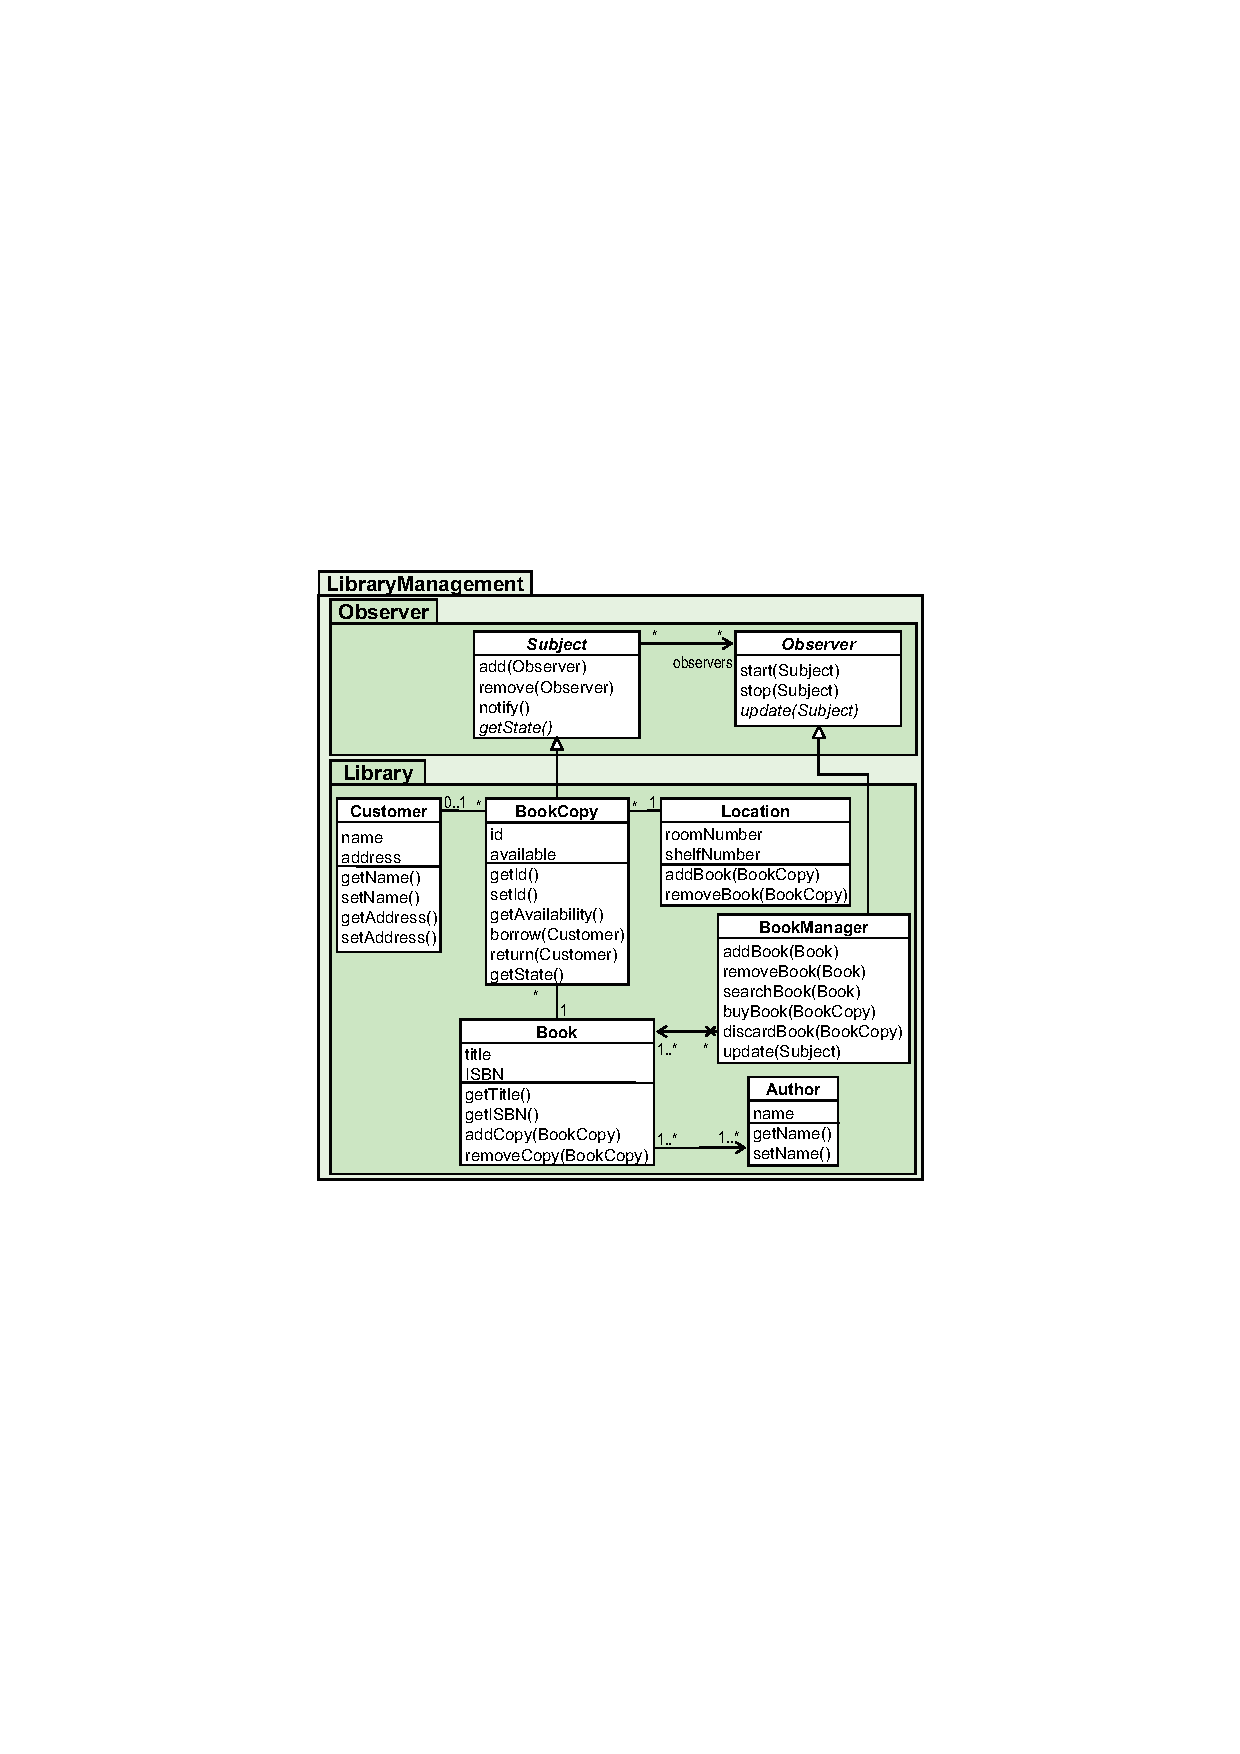
\includegraphics[width=0.7\textwidth]{figures/figure1}
	\caption{Sample figure}
	\label{fig:samplefigure_pdf}
\end{figure}


\section{Fonts}

When introducing important terms for the first time use \emph{emphasize}. For a consistent look and feel of proper names like {\cd} and {\uml{Observer}} pattern you may define macros in the main document \texttt{thesis.tex}.

\section{Code}

For short code fragments use the \textit{verbatim} environment.

\begin{verbatim}
//Start Program
System.out.println("Hello World!");
//End Program
\end{verbatim}

A much better alternative is the \textit{algorithm} environment (cf. Algorithm~\ref{alg:samplealgorithm}). This environment offers special formatting features for loops, operations and comments.

\begin{algorithm}[t]
\SetKwData{Left}{left}
\SetKwData{This}{this}
\SetKwData{Up}{up}
\SetKwFunction{Union}{Union}
\SetKwFunction{FindCompress}{FindCompress}
\SetKwInOut{Input}{input}
\SetKwInOut{Output}{output}

\Input{A bitmap $Im$ of size $w\times l$}
\Output{A partition of the bitmap}

\BlankLine

\emph{special treatment of the first line}\;
\For{$i\leftarrow 2$ \KwTo $l$}{
\emph{special treatment of the first element of line $i$}\;
\For{$j\leftarrow 2$ \KwTo $w$}{\label{forins}
\Left$\leftarrow$ \FindCompress{$Im[i,j-1]$}\;
\Up$\leftarrow$ \FindCompress{$Im[i-1,]$}\;
\This$\leftarrow$ \FindCompress{$Im[i,j]$}\;
\If(\tcp*[r]{O(\Left,\This)==1}){\Left compatible with \This}{\label{lt}
\lIf{\Left $<$ \This}{\Union{\Left,\This}}\;
\lElse{\Union{\This,\Left}\;}
}
\If(\tcp*[r]{O(\Up,\This)==1}){\Up compatible with \This}{\label{ut}
\lIf{\Up $<$ \This}{\Union{\Up,\This}}\;
\tcp{\This is put under \Up to keep tree as flat as possible}\label{cmt}
\lElse{\Union{\This,\Up}}\tcp*[r]{\This linked to \Up}\label{lelse}
}
}
\lForEach{element $e$ of the line $i$}{\FindCompress{p}}
}
\caption{Sample algorithm}\label{alg:samplealgorithm}
\end{algorithm}



%%%%%%%%%%%%%%%%%%%%%%%%%%%%%%%%%%%%%%%%%
\chapter{Bibliographic Issues}
\label{ch:bibliographic}
%%%%%%%%%%%%%%%%%%%%%%%%%%%%%%%%%%%%%%%%%

\section{Literature Research}

%Information on online libraries and literature search, e.g., interesting magazines, journals, conferences, and organizations may be found at \url{http://www.big.tuwien.ac.at/teaching/info.html}.
%
%\section{BibTeX}
%
%BibTeX should be used for referencing.
%
%The LaTeX source document of this pdf document provides you with different samples for references to journals~\cite{jour:B2BServices}, conference papers~\cite{proc:TheWebMLApproach}, books~\cite{book:umlatwork}, book chapters~\cite{incoll:ErhardKonrad1992}, electronic standards~\cite{man:BPEL}, dissertations~\cite{phdthesis:manuelWimmer}, masters' theses~\cite{mast:AUMLProfile}, and web sites~\cite{misc:BIGWebsite}. The respective BibTeX entries may be found in the file \texttt{references.bib}. For administration of the BibTeX references we recommend \url{http://www.citeulike.org} or JabRef for offline administration, respectively.


%%%%%%%%%%%%%%%%%%%%%%%%%%%%%%%%%%%%%%%%%
%%% BACKMATTER %%%%%%%%%%%%%%%%%%%%%%%%%%
%%%%%%%%%%%%%%%%%%%%%%%%%%%%%%%%%%%%%%%%%

\appendix

\bibliographystyle{plain}
\bibliography{references}

\end{document}
